\chapter{System Design}

The design of the \textbf{CricketVision: AI-Powered Cricket Performance Analytics and Biomechanics Platform} describes the overall structure, data flow, and working sequence of the application. The design is based on the requirements identified during the system study and represents how the major components of the application interact with the user and with each other. The main design representations used in this project are the system design, Data Flow Diagram Level 0, Data Flow Diagram Level 1, and system workflow.

\section{System Design}
The CricketVision platform is designed as a web-based application consisting of a frontend, application layer, database, and processing components. The user interacts with the system through the frontend interface. The application layer handles the major operations such as authentication, roster management, statistical processing, SVG wagon wheel rendering, match simulation, video pose analysis, and AI Coach advice generation.

The frontend communicates with the backend through REST APIs. The backend manages application operations and communicates with the database for storing and retrieving user and player information. Player profiles are auto-seeded on deployment, and video playback feeds are processed using canvas rendering engines to calculate joint flexion angles.

The structured player information can be reused by different modules of the application. For example, the same player profile data can be used for phase-wise statistical breakdowns, 360-degree SVG wagon wheel rendering, stochastic match simulation, and AI strategy advice generation. This reduces repeated data entry and provides a common source of information for the different functions.

The major components represented in the system design are:
\begin{itemize}
    \item \textbf{Presentation Layer (Client):} Built using React 18, Vite, and Tailwind CSS. Provides the user interface, renders SVG wagon wheels, displays Recharts radar charts, overlays video pose skeletons, and sends API requests to the backend.
    \item \textbf{Application Layer (Server):} Built using Node.js and Express.js REST APIs. Handles authentication, roster management controllers, stochastic match simulation logic, and AI Coach processing.
    \item \textbf{Data Layer (Persistence):} Powered by MongoDB and Mongoose ODM. Stores user credentials and 100+ structured player documents.
    \item \textbf{AI \& Biomechanics Processing:} Google Gemini API for natural language strategy advice and HTML5 canvas keypoint calculation for joint flexion auditing.
\end{itemize}

\begin{figure}[H]
\centering
\begin{tikzpicture}[
  node distance=1.8cm, auto,
  block/.style={rectangle, draw=blue!80!black, fill=blue!5, thick, text width=10.2cm, align=center, rounded corners=4pt, minimum height=1.3cm, font=\small},
  arrow/.style={draw=blue!80!black, ->, >=stealth, thick}
]

  \node [block] (frontend) {\textbf{\mbox{PRESENTATION LAYER (REACT 18 \& VITE)}}\\Coach Dashboard \quad$|$\quad Player Portal \quad$|$\quad Analyst Simulator \quad$|$\quad Pose Analyzer};
  \node [block, below=of frontend] (backend) {\textbf{\mbox{APPLICATION LAYER (EXPRESS.JS \& NODE.JS)}}\\Auth Router \quad$|$\quad Player Controller \quad$|$\quad Match Simulator Engine \quad$|$\quad AI Coach};
  \node [block, below=of backend] (database) {\textbf{\mbox{DATA LAYER (MONGODB 6.0+)}}\\Collection: \texttt{players} (104 Docs) \quad$|$\quad Collection: \texttt{users} (Role Presets)};

  % Left Downward Arrow: Requests (Presentation -> Application)
  \draw [arrow] ([xshift=-3.2cm] frontend.south) -- node[left, font=\footnotesize, fill=white, inner sep=2pt] {HTTP Requests (API)} ([xshift=-3.2cm] backend.north);

  % Left Downward Arrow: Queries (Application -> Data)
  \draw [arrow] ([xshift=-3.2cm] backend.south) -- node[left, font=\footnotesize, fill=white, inner sep=2pt] {Mongoose Queries} ([xshift=-3.2cm] database.north);

  % Right Upward Arrow: Data Streams (Data -> Application)
  \draw [arrow] ([xshift=3.2cm] database.north) -- node[right, font=\footnotesize, fill=white, inner sep=2pt] {Document Stream} ([xshift=3.2cm] backend.south);

  % Right Upward Arrow: JSON Payload (Application -> Presentation)
  \draw [arrow] ([xshift=3.2cm] backend.north) -- node[right, font=\footnotesize, fill=white, inner sep=2pt] {JSON Payload} ([xshift=3.2cm] frontend.south);

\end{tikzpicture}
\caption{System Design of CricketVision Platform}
\label{fig:system_design}
\end{figure}

The system design provides an overall view of the major components and their interaction within the application. It forms the basis for understanding the detailed data flow and workflow represented in the following diagrams.

\section{Data Flow Diagram - Level 0}
The Level 0 Data Flow Diagram provides a high-level representation of the proposed system. In this diagram, the complete application is represented as a single process and the interaction between the user entities (Head Coach, Elite Player, Sports Analyst) and the system is shown.

The user provides different types of information such as authentication credentials, roster edits, match simulation parameters, and video playback files. The system processes these inputs and provides outputs such as phase-wise stats, wagon wheel heatmaps, win-probability curves, pose flex angle audits, and AI strategy advice.

The Level 0 DFD focuses on the overall boundary of the system and does not describe the internal processing activities in detail. It provides a simple representation of the relationship between the user roles and the complete application.

\begin{figure}[H]
\centering
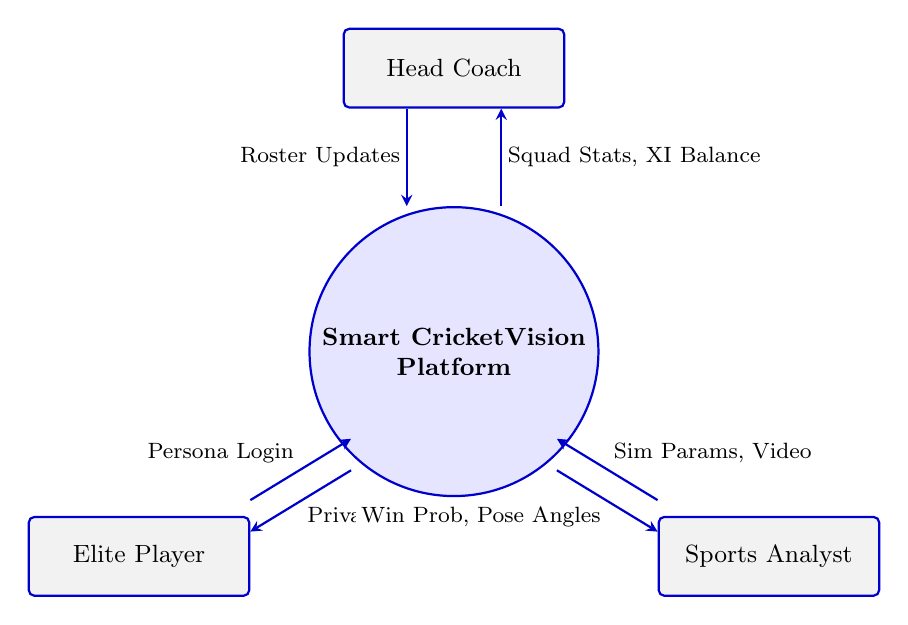
\begin{tikzpicture}[
  entity/.style={rectangle, draw=blue!80!black, fill=gray!10, thick, minimum width=2.8cm, minimum height=1.0cm, align=center, rounded corners=2pt, font=\small},
  process/.style={circle, draw=blue!80!black, fill=blue!10, thick, minimum size=2.8cm, align=center, font=\small},
  arrow/.style={draw=blue!80!black, ->, >=stealth, thick}
]

  % Central Process
  \node [process] (system) at (0,0) {\textbf{Smart CricketVision}\\\textbf{Platform}};
  
  % Top Entity (Head Coach)
  \node [entity] (coach) at (0, 3.6) {Head Coach};
  
  % Bottom Left Entity (Elite Player)
  \node [entity] (player) at (-4.0, -2.6) {Elite Player};
  
  % Bottom Right Entity (Sports Analyst)
  \node [entity] (analyst) at (4.0, -2.6) {Sports Analyst};

  % --- Head Coach Connections ---
  \draw [arrow] ([xshift=-0.6cm] coach.south) -- node[left, font=\footnotesize, fill=white, inner sep=2pt] {Roster Updates} ([xshift=-0.6cm] system.north);
  \draw [arrow] ([xshift=0.6cm] system.north) -- node[right, font=\footnotesize, fill=white, inner sep=2pt] {Squad Stats, XI Balance} ([xshift=0.6cm] coach.south);

  % --- Elite Player Connections ---
  \draw [arrow] ([yshift=0.2cm] player.north east) -- node[above left, font=\footnotesize, fill=white, inner sep=2pt] {Persona Login} ([yshift=0.2cm] system.south west);
  \draw [arrow] ([yshift=-0.2cm] system.south west) -- node[below right, font=\footnotesize, fill=white, inner sep=2pt] {Private Form, Drills} ([yshift=-0.2cm] player.north east);

  % --- Sports Analyst Connections ---
  \draw [arrow] ([yshift=0.2cm] analyst.north west) -- node[above right, font=\footnotesize, fill=white, inner sep=2pt] {Sim Params, Video} ([yshift=0.2cm] system.south east);
  \draw [arrow] ([yshift=-0.2cm] system.south east) -- node[below left, font=\footnotesize, fill=white, inner sep=2pt] {Win Prob, Pose Angles} ([yshift=-0.2cm] analyst.north west);

\end{tikzpicture}
\caption{Data Flow Diagram - Level 0}
\label{fig:dfd_level0}
\end{figure}

The Level 0 DFD gives an overview of the major input and output flow of the application. The internal processes involved in handling these data flows are represented in the Level 1 DFD.

\section{Data Flow Diagram - Level 1}
The Level 1 Data Flow Diagram provides a detailed representation of the major processes within the CricketVision platform. The complete system is divided into individual processes so that the movement of information between the user, application processes, and database can be understood clearly.

The major processes represented in the Level 1 DFD are:
\begin{enumerate}
    \item \textbf{User Authentication:} Handles persona preset selection and credential login verification.
    \item \textbf{Roster Management \& Player Seeding:} Accepts manual player edits and automatically seeds 104 verified player profiles.
    \item \textbf{Visual Analytics Processing:} Transforms polar shot coordinates into Cartesian SVG wagon wheel heatmaps.
    \item \textbf{Stochastic Match Simulation:} Evaluates target scores, pitch factors, and weather to calculate win-probability curves.
    \item \textbf{Video Pose Biomechanics Analysis:} Processes video keypoints to compute elbow flex angles and audit ICC compliance.
    \item \textbf{AI Coach Strategy Generation:} Evaluates squad stats and fatigue indicators to produce natural language recommendations.
\end{enumerate}

\begin{figure}[H]
\centering
\begin{tikzpicture}[
  entity/.style={rectangle, draw=blue!80!black, fill=gray!15, thick, minimum width=2.4cm, minimum height=0.9cm, align=center, rounded corners=2pt, font=\small},
  process/.style={ellipse, draw=blue!80!black, fill=blue!10, thick, minimum width=2.8cm, minimum height=1.2cm, align=center, font=\small},
  store/.style={rectangle, draw=green!60!black, fill=green!5, thick, minimum width=2.4cm, minimum height=0.85cm, align=center, font=\small},
  arrow/.style={draw=blue!80!black, ->, >=stealth, thick}
]

  % Single Left Entity (x = -4.0)
  \node [entity] (user) at (-4.0, 0) {User / Actor};

  % Processes Stacked Cleanly in Middle Column (x = 0)
  \node [process] (p1) at (0,  3.0) {\textbf{1.0}\\Authenticate User};
  \node [process] (p2) at (0,  1.0) {\textbf{2.0}\\Manage Roster};
  \node [process] (p3) at (0, -1.0) {\textbf{3.0}\\Match Simulation};
  \node [process] (p4) at (0, -3.0) {\textbf{4.0}\\Pose Biomechanics};

  % Data Stores Stacked Cleanly in Right Column (x = 4.0)
  \node [store] (d1) at (4.0,  3.0) {D1: Users DB};
  \node [store] (d2) at (4.0,  1.0) {D2: Players DB};
  \node [store] (d3) at (4.0, -1.0) {D3: Match Logs DB};

  % Arrows from User to Processes
  \draw [arrow] (user.east) -- (p1.west);
  \draw [arrow] (user.east) -- (p2.west);
  \draw [arrow] (user.east) -- (p3.west);
  \draw [arrow] (user.east) -- (p4.west);

  % Arrows from Processes to Stores
  \draw [arrow] (p1.east) -- (d1.west);
  \draw [arrow] (p2.east) -- (d2.west);
  \draw [arrow] (p3.east) -- (d3.west);

\end{tikzpicture}
\caption{Data Flow Diagram - Level 1}
\label{fig:dfd_level1}
\end{figure}

The Level 1 DFD provides a detailed view of how the major functional processes exchange information. It also shows how stored player information is reused by visual analytics, stochastic simulation, pose analysis, and AI strategy advice generation.

\section{System Workflow}
The system workflow represents the sequence of major activities available to the user. The user first registers or logs in using a persona preset and then accesses the dashboard. From the dashboard, the user can independently select the required function according to the purpose for which the application is being used.

The first major function is roster management, where the user views or edits player information and monitors workload fatigue alerts. Another function is visual analytics, where phase-wise stats, 360-degree SVG wagon wheels, and pitch length plots are displayed.

The third major function is stochastic match simulation. The user inputs target scores and match conditions to generate real-time win-probability curves.

The fourth major function is video pose analysis, where bowling action video feeds are audited for elbow flex compliance. The user can also access the AI Coach modal for tactical squad advice.

These functions are independent options available from the dashboard. The user is therefore not required to follow a fixed sequence through all the functions.

\begin{figure}[H]
\centering
\begin{tcolorbox}[diagrambox, title={System Workflow of CricketVision Platform}]
\begin{tikzpicture}[
  node distance=0.9cm and 0.2cm, auto,
  flowstep/.style={rectangle, draw=blue!80!black, fill=yellow!15, thick, rounded corners, text width=3.8cm, align=center, font=\small},
  decision/.style={diamond, draw=red!80!black, fill=red!10, thick, align=center, aspect=2, font=\small},
  circleend/.style={circle, draw=black, fill=black, inner sep=2.5pt},
  arrow/.style={draw=blue!80!black, ->, >=stealth, thick}
]

  \node [flowstep] (start) {\textbf{START: Register / Login}};
  \node [flowstep, below=of start] (dash) {\textbf{Access Central Dashboard}};
  
  \node [flowstep, below left=1.2cm and 0.1cm of dash] (f1) {Manage Roster \& Seeding};
  \node [flowstep, below=of dash] (f2) {Stochastic Match Simulation};
  \node [flowstep, below right=1.2cm and 0.1cm of dash] (f3) {Pose Video Biomechanics};
  
  \node [flowstep, below=of f1] (o1) {Phase Stats \& SVG Wagon Wheel};
  \node [flowstep, below=of f2] (o2) {Dynamic Win Prob Curve};
  \node [flowstep, below=of f3] (o3) {ICC Compliance Audit \& AI Advice};

  \draw [arrow] (start) -- (dash);
  \draw [arrow] (dash) -- (f1);
  \draw [arrow] (dash) -- (f2);
  \draw [arrow] (dash) -- (f3);
  \draw [arrow] (f1) -- (o1);
  \draw [arrow] (f2) -- (o2);
  \draw [arrow] (f3) -- (o3);

\end{tikzpicture}
\end{tcolorbox}
\caption{System Workflow of CricketVision Platform}
\label{fig:system_workflow}
\end{figure}

The workflow provides a simple representation of the main user activities and the functions available through the dashboard. It shows the relationship between roster management, visual analytics, match simulation, pose biomechanics, and AI strategy advice.

\section{Design Summary}
The design of the CricketVision platform provides a clear representation of the structure and operation of the application. The system design describes the major components of the application and their interaction. The Level 0 DFD provides a high-level representation of the system, while the Level 1 DFD describes the major internal processes and data movement.

The system workflow represents the main functions available to the user from the dashboard. Together, these design representations provide the required view of the application structure, data flow, and user interaction. The design also supports the reuse of structured player information across statistical analytics, SVG wagon wheel rendering, match simulation, pose analysis, and AI strategy advice generation.
